\section{Preliminaries}
\label{sec:HomographyPreliminaries}

This section contains a description of our custom terminology. Despite the existence of standard conventions for naming certain aspects of our problem, we nevertheless had to coin a few more terms for clarity.

We define a marker as an object with a known, easy-to-detect shape. Such object can be either naturally occurring or artificially placed on the planar surface of the scene we want to remove perspective distortion from, i.e., to produce a bird's-eye view. The marker contains keypoints, which is a set of distinct, independent, visual feature points (for instance, corners). The chosen keypoints visible in the perspectively deformed image are called the \mbox{warped keypoints}. The set of the \mbox{rectified keypoints} is represented in the desired image (not subjected to perspective distortion) and is produced from the warped keypoints using the homography projection. Last but not least, the \mbox{point correspondence} is a relationship between the warped and the \mbox{target keypoints} and it is necessary for homography estimation. In an ideal case, the rectified keypoints match the target keypoints in terms of their pixel positions (see \figstr{}~\ref{fig:HomographyTerminology}).

\begin{figure}[t]
    \centering
    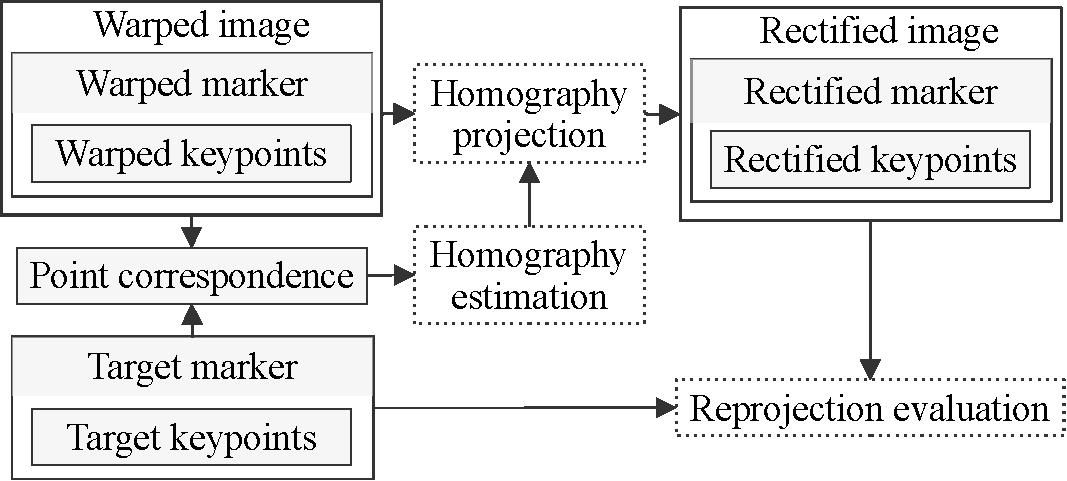
\includegraphics[width=0.6\linewidth]{figures/homography/terminology.pdf}
    \caption{Visualization of relationships within our established terminology. This diagram also depicts the hierarchical dependence between individual terms. In addition, the dotted elements represent processes with arrows denoting their input and output.}
    \label{fig:HomographyTerminology}
\end{figure}

Unless stated otherwise, a \mbox{\textbf{similarity transformation}} denotes a limited affine transformation with $4$ DoF which encompasses translation, rotation and uniform scaling (equation \eqref{eq:SimilarityMatrices}). Specifically, let $\mset{K}_1$ and $\mset{K}_2$ be sets of feature keypoints belonging to objects $O_1$ and $O_2$. We refer to the objects $O_1$ and $O_2$ as \mbox{\textbf{similar}} if there exists a similarity transformation $\psi$, such that $\mset{K}_1 = \func{\psi}{\mset{K}_2}$ and $\mset{K}_2 = \func{\psi^{-1}}{\mset{K}_1}$. For instance, $O_1$ and $O_2$ may represent rectangles of different sizes whilst having a equal aspect ratio.

Let $m$ denote the number of markers and $k$ represent the number of keypoints belonging to each marker in consideration. We describe each $i$-th marker using a $3 \times k$ matrix $\suprbrackets{\mtx{W}}{i}$ that stores the warped keypoints as
\begin{equation}
    \suprbrackets{\mtx{W}}{i} =
    \begin{bmatrix}
        \subsuprbrackets{x}{1}{i} & \subsuprbrackets{x}{2}{i} & \dots & \subsuprbrackets{x}{k}{i} \\
        \subsuprbrackets{y}{1}{i} & \subsuprbrackets{y}{2}{i} & \dots & \subsuprbrackets{y}{k}{i} \\
        1                         & 1                         & \dots & 1
    \end{bmatrix},
    i = 1, \dots, m.
\end{equation}
Analogivally, we describe the target keypoints using a $3 \times k$ matrix $\mtx{T}$. Owing to the many-to-one point correspondence, only one specification is sufficient. Just beware that the ordering of keypoints had to match the warped keypoints defined above, so
\begin{equation}
    \mtx{T} =
    \begin{bmatrix}
        \tilde{x}_1 & \tilde{x}_2 & \dots & \tilde{x}_k \\
        \tilde{y}_1 & \tilde{y}_2 & \dots & \tilde{y}_k \\
        1           & 1           & \dots & 1
    \end{bmatrix},
\end{equation}
with the point correspondence relationship formulated as
\begin{equation}
    \subsuprbrackets{x}{j}{i} \simeq \tilde{x}_j, \subsuprbrackets{y}{j}{i} \simeq \tilde{y}_j, i = 1, \dots, m, j = 1, \dots, k.
\end{equation}
